\chapterimage{Water1.png} % Chapter heading image

\chapter{Wastewater Math - Part I}

\section{Units}\index{Units}

To measure any quantity or compare two physical quantities we need a universally accepted standard called Unit. The most common measurements involve measuring - length, weight and time.   International System of Units (SI), the modern form of the metric system is the globally accepted standard.  In the United States, it is customary to measure the physical quantities in English Engineering Units.\\
\vspace{0.5cm}
\begin{tabular}{c c c }
\hline
\multicolumn{3}{c}{\textbf{Fundamental Units}} \\
\hline
\textbf{Dimension} & \textbf{English Engineering Units} & \textbf{SI}\\
\hline
time & second (s) & second (s) \\
length & foot (ft) & meter (m)\\
mass & pound mass (lb) & kilogram\\
\end{tabular}\\

\vspace{0.5cm}

The measurement of any physical quantity is expressed in terms of a number - which is the quantity and a specific unit.  
Thus, a measurement of 5000 ft is basically 5000 of the of length as measured in ft.

Using the fundamental physical measurements, mathematical calculations can be made to measure other physical quantities such as area (ft$2$), volume (ft$3$), velocity (ft/s), flow (ft$3$/s), density (lbs/ft$3$).

Depending on the what is being measured or quantified, there are appropriate and customary units of measure - for example - miles and inches for length, gallons and acre-ft for volume and milligrams and tons for mass.
% \begin{enumerate}
% \definecolor{shadecolor}{RGB}{200, 200, 240}
% \begin{snugshade*}
%\section{Units and Unit Conversion}\index{Units and Unit Conversion}
% 	\item \noindent\textsc{Units and Unit Conversion}
% \end{snugshade*}
\subsection{Unit Conversions}\index{Unit Conversions}
Unit conversion is a process for changing the units of a measured quantity without changing its value.  It involves 
utilizing a \hl{conversion factor} which expresses the relationship between units that is used to change the units of a measured quantity without changing the value. Examples of conversion factors include:\\

\begin{center}
\renewcommand{\arraystretch}{1.5}
\vspace{0.5cm}
\begin{tabular}{l| c c }
\hline
\multicolumn{2}{c}{\textbf{Fundamental Units}} \\
\hline
\textbf{Dimension} & \textbf{Conversion Factor}\\[0.5cm]

\hspace{0.3cm}
time & $\dfrac{60 \enspace sec}{min}$, $\dfrac{1,440\enspace sec}{day}$\\[0.5cm]
length & $\dfrac{12 \enspace in}{ft}$, $\dfrac{5,280 \enspace ft}{mile}$\\[0.5cm]
mass & $\dfrac{2,000 \enspace lbs}{ton}$, $\dfrac{1000 \enspace gm}{mg}$\\
\end{tabular}\\
\begin{tabular}{l| c c }
\hline
\multicolumn{2}{c}{\textbf{Derived Units}} \\
\hline
\textbf{Dimension} & \textbf{Conversion Factor}\\[0.5cm]

\hspace{0.3cm}
area & $\dfrac{43,560 \enspace ft^2}{acre}$, $\dfrac{60 \enspace sec}{min}$\\[0.5cm]
volume & $\dfrac{27 \enspace ft^3}{yd}$, $\dfrac{7.48 \enspace gal}{ft^3}$\\
\end{tabular}\\
\end{center}
\vspace{0.5cm}

The numerator and the denominator of any conversion factor always equals one, they have the same value expressed in different units.

For converting one measurement unit to another.

Step 1:  Make sure the original unit is for the same measurement as the conversion unit.  So if the original unit is for area, say ft$^2$ the conversion unit can be another area unit such as in$^2$ or acre but it cannot be gallons as gallon is a unit of volume.

Step 2: Write down the conversion formula as:

$Quantity \enspace in \enspace converted \enspace unit = Quantity \enspace (\cancel{Original \enspace Unit}) *   Conversion  \enspace Factor \enspace  \dfrac{Conversion \enspace unit}{\cancel{Original \enspace unit}}$\\
\hspace{0.2cm}
Unit conversions may involve single factor where the original unit value is multiplied by the conversion factor to obtain the measured parameter in the converted (desired) unit.\\
For example:\\  
Converting 1000 $ft^3$ to cu. yards:\\

$1000 \cancel{ft^3}*\dfrac{cu.yards}{27\cancel{ft^3}} = 37 cu.yards$\\

Other unit conversions may require multiplying by known constants along with conversion factors.\\
For example:\\
\begin{enumerate}  

\item Converting 3.5 $ft^3/sec$ to MGD:\\
$\dfrac{3.5 \enspace \cancel{ft^3}}{\cancel{sec}} * \dfrac{7.48\cancel {\enspace gal}}{\cancel{ft^3}} * \dfrac{MG}{\enspace 10^6 \cancel{gal}}* \dfrac{1440*60 \enspace \cancel{sec}}{day}=  2.3 \enspace MGD$\\

\item Converting 1,000 L water to lbs:\\
$1000 \enspace \cancel{L}*\dfrac {\cancel{gal}}{3.785 \enspace \cancel{L}}*\dfrac{8.34 \enspace lbs}{\cancel{gal}}\enspace  = 2,203 \enspace lbs$\\
$(Note:8.34 \enspace lbs/gal \enspace is \enspace density \enspace of \enspace water - a \enspace constant)$\\ 

\end{enumerate}

\section{Area \& Volume}\index{Area \& Volume}
% \section{Area \& Volume}\index{Area \& Volume}

% \begin{snugshade*}
% 	\item \noindent\textsc{Area \& Volume}
% \end{snugshade*}

\begin{center}
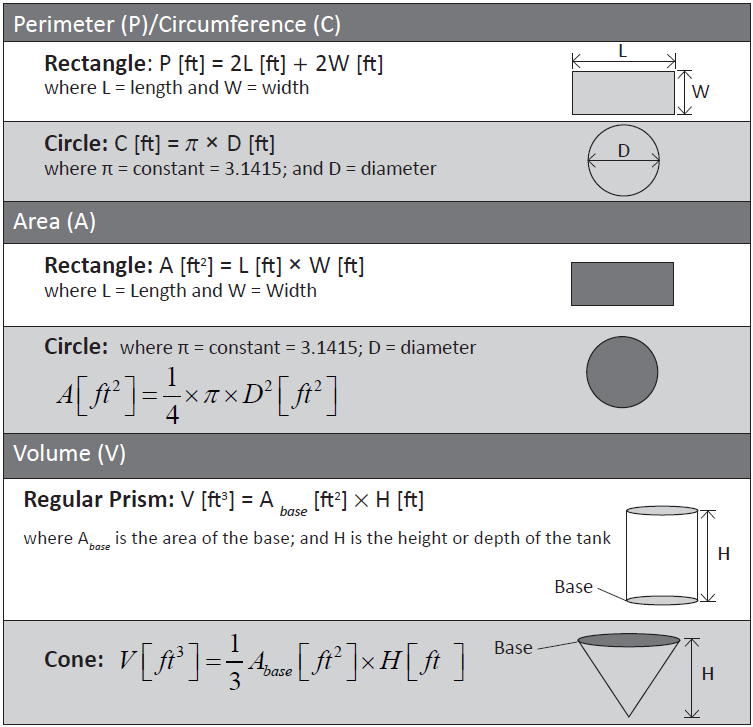
\includegraphics[scale=0.5]{Area&VolumeFormula}
\end{center}
\subsection{Example Problems}
% \hl{Example Problems}\\
\begin{enumerate}

\item The floor of a rectangular building is 20 feet long by 12 feet wide and the inside walls are 10 feet high. Find the total surface area of the inside walls of this building\\
Solution:\\
% \begin{center}
\begin{tikzpicture}
	%%% Edit the following coordinate to change the shape of your
	%%% cuboid
      
	%% Vanishing points for perspective handling
	\coordinate (P1) at (-7cm,1.5cm); % left vanishing point (To pick)
	\coordinate (P2) at (8cm,1.5cm); % right vanishing point (To pick)

	%% (A1) and (A2) defines the 2 central points of the cuboid
	\coordinate (A1) at (0em,0cm); % central top point (To pick)
	\coordinate (A2) at (0em,-2cm); % central bottom point (To pick)

	%% (A3) to (A8) are computed given a unique parameter (or 2) .8
	% You can vary .8 from 0 to 1 to change perspective on left side
	\coordinate (A3) at ($(P1)!.8!(A2)$); % To pick for perspective 
	\coordinate (A4) at ($(P1)!.8!(A1)$);

	% You can vary .8 from 0 to 1 to change perspective on right side
	\coordinate (A7) at ($(P2)!.7!(A2)$);
	\coordinate (A8) at ($(P2)!.7!(A1)$);

	%% Automatically compute the last 2 points with intersections
	\coordinate (A5) at
	  (intersection cs: first line={(A8) -- (P1)},
			    second line={(A4) -- (P2)});
	\coordinate (A6) at
	  (intersection cs: first line={(A7) -- (P1)}, 
			    second line={(A3) -- (P2)});

	%%% Depending of what you want to display, you can comment/edit
	%%% the following lines

	%% Possibly draw back faces

	\fill[gray!40] (A2) -- (A3) -- (A6) -- (A7) -- cycle; % face 6
	\node at (barycentric cs:A2=1,A3=1,A6=1,A7=1) {\tiny Floor=W*L};
	
	\fill[gray!50] (A3) -- (A4) -- (A5) -- (A6) -- cycle; % face 3
	\node at (barycentric cs:A3=1,A4=1,A5=1,A6=1) {\tiny Wall - W*H};
	
	\fill[gray!10, opacity=0.2] (A5) -- (A6) -- (A7) -- (A8) -- cycle; % face 4
	\node at (barycentric cs:A5=1,A6=1,A7=1,A8=1) {\tiny Wall - L*H};
	
	\fill[gray!10,opacity=0.5] (A1) -- (A2) -- (A3) -- (A4) -- cycle; % f2
	\node at (barycentric cs:A1=1,A2=1,A3=1,A4=1) {\tiny Wall - L*H};
	
	\fill[gray!40,opacity=0.2] (A1) -- (A4) -- (A5) -- (A8) -- cycle; % f5
	\node at (barycentric cs:A1=1,A4=1,A5=1,A8=1) {\tiny Ceiling=W*L};	
	
	\draw[thick,dashed] (A5) -- (A6);
	\draw[thick,dashed] (A3) -- (A6);
	\draw[thick,dashed] (A7) -- (A6);

	%% Possibly draw front faces

	%\fill[orange] (A1) -- (A8) -- (A7) -- (A2) -- cycle; % face 1
	\node at (barycentric cs:A1=1,A8=1,A7=1,A2=1) {\tiny Wall - W*H};
	


	%% Possibly draw front lines
	\draw[thick] (A1) -- (A2);

	\draw[<->] (-1.8,0.38) -- (-1.8,-1.3)node [midway, above=-1.8mm] {\hspace{-1.3cm}\tiny Height=10'};
	\draw[<->] (-1.6,-1.4) -- (-.3,-2.1)node [midway, above=-2.6mm] {\hspace{-1.3cm}\tiny Length=20'};
	\draw[<->] (2.6,-1.13) -- (0.2,-2.2)node [midway, below=.6mm] {\hspace{1.2cm}\tiny Width=12'};
	\draw[thick] (A3) -- (A4);
	\draw[thick] (A7) -- (A8);
	\draw[thick] (A1) -- (A4);
	\draw[thick] (A1) -- (A8);
	\draw[thick] (A2) -- (A3);
	\draw[thick] (A2) -- (A7);
	\draw[thick] (A4) -- (A5);
	\draw[thick] (A8) -- (A5);
	
	% Possibly draw points
	% (it can help you understand the cuboid structure)
%	\foreach \i in {1,2,...,8}
%	{
%	  \draw[fill=black] (A\i) circle (0.15em)
%	    node[above right] {\tiny \i};
%	}
	% \draw[fill=black] (P1) circle (0.1em) node[below] {\tiny p1};
	% \draw[fill=black] (P2) circle (0.1em) node[below] {\tiny p2};
\end{tikzpicture}\\
% \end{center}
2 Walls W*H + 2 Walls L*H= $2*12*10ft^2 + 2*20*10ft^2$\\
$=240+400=\boxed{640ft^2}$

2 Walls W*H + 2 Walls L*H + Floor + Ceiling= $2*12*10ft^2 + 2*20*10ft^2 + 2*12*20ft^2$\\
$=240+400+480=\boxed{1,120ft^2}$
\end{enumerate}
\section{Concentration}\index{Concentration}

Concentration is typically expressed as mg/l which is the weight of the constituent (mg) in 1 l (liter) of solution (wastewater).  As 1 l of water weighs 1 million mg, a concentration of 1 mg/l implies 1 mg of constituent per 1 million mg of water or one part per million (ppm).   \textbf{Thus, mg/l and ppm are synonymous.}\\  
Sometimes the constituent concentration is expressed in terms of percentage.\\
\vspace{6pt}
For example:  sludge containing 5\% solids or a 12.5\% chlorine concentration solution.\\
\vspace{6pt}
As one liter of water weighs 1,000,000 mg, one percent of that weight is 10,000 mg.  So 1\% solids implies 10,000 mg of solids per liter or 10,000 mg/l or 10,000 ppm.\\
\vspace{6pt}
$1\% concentration = 10,000 \enspace ppm \enspace or \enspace\dfrac{mg}{l}$\\
\vspace{6pt}
$0.1\% concentration = 1,000 \enspace ppm \enspace or \enspace \dfrac{mg}{l}$\\
\vspace{6pt}
$0.01\% concentration = 100 \enspace ppm \enspace or \enspace \dfrac{mg}{l}$\\
\vspace{6pt}
$10\% concentration = 100,000 \enspace ppm \enspace or \enspace \dfrac{mg}{l}$\\
\vspace{6pt}
$5\% concentration = 50,000 \enspace ppm \enspace or \enspace \dfrac{mg}{l}$\\
\vspace{6pt}
$A \enspace  12.5\% \enspace bleach \enspace solution \enspace contains \enspace 12.5\% \enspace or \enspace 125,000 \enspace \dfrac{mg}{l} \enspace of \enspace \enspace active \enspace chlorine $

